\chapter{Соревнования  «Гонки», RobotC}
{\bfseries Анонс:}\\\\
Соревнования «Гонки». Анализ технических решений. Проблемы командного взаимодействия. Языки программирования. Среда программирования RobotC. Общая структура программы.\\\\
{\bfseries Цели:}
\begin{itemize}
	\item{}{\bfseries Обучающие:} Повторение понятий передаточное соотношение, повышающая передача. Развитие навыков простейшего конструирования. Закрепление  принципов устойчивости конструкций. Знакомство с редактором RobotC.
	\item{}{\bfseries Коммуникативная:} Обучение детей работать во взаимодействии с другими учащимися (работа в группах) и учителем.\\
\end{itemize}	
{\bfseries Ход занятия:}\\\\
\begin{tabular}{lll}
	\hyperlink{lesson9x1}{1. Организационный момент} & Презентация & (5 мин)\\
	\hyperlink{lesson9x2}{2. Соревнования «Гонки»} & Игра & (50 мин) \\
	\hyperlink{lesson9x3}{3. Анализ технических решений} & Рефлексия & (15 мин) \\
	\hyperlink{lesson9x4}{4. Проблемы командного взаимодействия} & Рефлексия & 10 мин)\\
	\hyperlink{lesson9x5}{5. Языки программирования.Среда RobotC} & Презентация & 15 мин)\\
	\hyperlink{lesson9x6}{6. Практикум «Ленивая программа»} & Практика & 15 мин)\\
\end{tabular}\\\\

{\hypertarget{lesson9x1}{\blackBlueText{I. Организационный момент}}}\\\\ 

Первая часть занятия пройдет в режиме соревнований команд, каждой команде понадобиться свое рабочее место с набором и компьютером. Помимо этого следует выделить место под испытательный полигон, где дети смогут протестировать своих робот и засечь их результаты.

Во второй части занятия преподавателю потребуется проектор, а каждому учащемуся~--- компьютер с RobotC и блок NXT.\\\\

{\hypertarget{lesson9x2}{\blackBlueText{II.   Соревнования «Гонки» }}}\\\\

Учащиеся делятся на команды по 2--3 человека. Каждой команде предлагается придумать свое название, все команды вносятся в турнирную таблицу (рисуется на доске или проецируется на экран с компьютера).
Каждая команда получает задание~--- за 20 минут собрать гоночного робота, который быстрее всего преодолеет прямой участок трассы.\\\\
{\bfseries Регламент состязаний:}

\begin{enumerate}
	\item Программа робота пишется на блоке, одинакова для всех участников и представляет собой: Forward\(\to\)Empty\(\to\)Forward\(\to\)Empty\(\to\)Loop.
	\item По команде «Старт» участники запускаю программу на своих роботах. После этого вмешиваться в работу роботов любыми способами  запрещено!
	\item Роботы должны преодолеть ровный горизонтальный участок, протяженностью 10 метров.
	\item У каждой команды есть 3 попытки. В зачет идет лучший результат.
	\item Перерыв между попытками составляет не менее 5 минут.
	\item Победа присуждается роботу, показавшему лучшее время по результатам трех попыток.\\\\
\end{enumerate}

{\hypertarget{lesson9x3}{\blackBlueText{III. Анализ технических решений}}}\\\\

\begin{enumerate}
	\item Использовали ли вы повышающую передачу?
	\item Каково было передаточное соотношение?
	\item Покажите ведущие колеса вашего робота? Где сосредоточена основная масса вашего робота?
	\item Почему вы думаете, робот ехал не совсем прямо?*
	\item Как можно добиться прямолинейного движения?*
\end{enumerate}

{\slshape *Эти вопросы, касающиеся разных условий движения и управления правого и левого колеса, рекомендуется обсуждать только в сильных группах. Поиск путей решения проблемы подводит детей к идеи подчинения ( синхронизации) моторов, которую можно подробнее обсудить уже при изучении команды syncMotor.}\\\\

{\hypertarget{lesson9x4}{\blackBlueText{IV. Проблемы командного взаимодействия}}}\\\\

\begin{enumerate}
	\item Как вы выбрали, чью модель гоночной машины реализовывать?
	\item Изучили ли вы оба решения прежде, чем выбрать? Было ли ваше итоговое решение комбинацией изначальных? Или вы придумали новое, оптимальное?
	\item Сложно ли было договориться друг с другом?
	\item Услышал ли ваши предложения ваш напарник?
	\item Как вы распределили обязанности в процессе построения робота?
	\item Изменяли ли вы конструкцию вашего робота в перерывах между попытками? Как вы договаривались, что стоит изменить?\\\\
\end{enumerate}

{\hypertarget{lesson9x5}{\blackBlueText{V. Языки программирования, среда RobotC}}}\\\\

Итак, наш робот умеет быстро ехать прямо. Хотелось бы научить его поворачивать, получать показания с датчиков, обрабатывать их. Одним словом, пора учить робота думать. Для этого мы должны дать процессору инструкции на понятном ему языке. Сам процессор, умеет лишь слепо, байт за байтом исполнять инструкции, которые ему подсунули. К примеру, следующая последовательность нулей и единиц 00001001 00000110 00011001  00101001 00000100 10000011 01000001 0010100000000110 10000011 00100001 заставит процессор вывести на экран надпись «АААА!». Довольно непонятный способ общения, согласитесь. К счастью, существует множество «переводчиков» с машинного языка.

Все программы пишутся на вполне понятном человеку языке (Assembler, C, C++, C\#, Java, Python): их ещё называют «исходным кодом», просто «кодом» или «исходниками». Они пишутся в простые текстовые файлы с помощью {\slshape любого} текстового редактора, хоть с помощью Блокнота. Затем они превращаются в понятные процессору наборы нулей и единиц с помощью компилятора: компилятор получает на вход исходный код, а на выходе создаёт {\slshape бинарный исполняемый файл}, тот самый, понятный процессору, состоящий из единиц и нулей.

\begin{figure}[h!]
	\begin{center}
		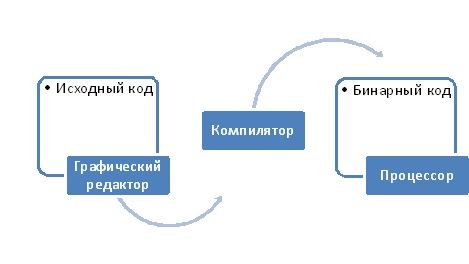
\includegraphics[width=0.75\linewidth]{chapters/chapter9/images/1}
		\caption{Принципиальная блок схема работы компилятора.}
		\label{ris:image9x1}
	\end{center}
\end{figure}

Для программирования микроконтроллера LegoMindstormsNXT 2.0 придуман целый ряд языков. Мы будем использовать язык компилятор {\slshape RobotC}  (для простоты в дальнейшем будем называть его просто {\slshape RobotC}) позволяющий создавать управляющие программы используя языки программирования C/С++.

{\slshape RobotC~--- интегрированная среда разработки (IDE), ориентированная на разработку программного обеспечения для микроконтроллеров NXT, входящих в набор Lego Mindstorms. В ней содержится набор необходимых функций для программирования, перепрошивки, отладки  и прочих действий с NXT, которые будут рассмотрены далее.
Бесплатную 30-дневную версию RobotC можно скачать с сайта \href{http://robotc.ru/}{http://robotc.ru/} . Для дальнейшего использования необходима покупка лицензии. После покупки лицензии вы получите на электронную почту подтверждение об этом, включающее код лицензии и пароль.

\begin{enumerate}
	\item Выберите пункт меню Help\(\to\)Manage Licenses
	\item В появившемся окне ROBOTC License Management, нажмите на кнопку "Add License"
	\item Выберите продукт, укажите полученный код лицензии и пароль
	\item Нажмите на кнопку Activate Online и ваши данные будут отправлены в службу поддержки ROBOTC. После того как служба поддержки получит и проверить эти данные, лицензия будет активирована автоматически.
\end{enumerate}}

Прежде всего, рекомендуется установить максимальный уровень интерфейса IDE (superuser). Для этого необходимо зайти в пункт меню Window\(\to\)MenuLevel и поставить галочку на пункте SuperUser. Далее возможны два варианта работы: работа с физическим роботом (режим работы, в котором созданный код может сразу же компилироваться и отправляться на контроллер робота), или же работа с эмулятором робота (режим в котором не происходит никакого взаимодействия с роботом). Для выбора соответствующего режима необходимо зайти в пункт меню Robot\(\to\)CompilerTargetи поставить галочку напротив соответствующего режима работы (PhysicalRobot или PC-BasedEmulator соответственно). Мы будем рассматривать только режим работы с физическим роботом.

{\slshape Удобно проводить объяснение и последующий практикум в следующем формате: учитель показывает действие на своем компьютере, подключенном к проектору, а затем каждый ребенок на своем компьютере повторяет операцию и задает вопросы, при необходимости.}

Сама программа пишется во встроенном текстовом редакторе, который имеет вид, представленный на рис.~\ref{ris:image9x1} Кроме самого редактора (1), есть два удобных вспомогательных окна: (2) окно вывода информации о компиляции (errors, warnings, и т.д., т.е. проблемы, возникшие у компилятора при переводе программы на понятный машине язык)  и (3)  окно быстрой справки по функционалу библиотеки. В нем описаны шапки стандартных функций и переменных, а так же есть ссылки в локальную справку. При компиляции, отправки кода на робота и запуске его там, не разрывая соединения с компьютером, это окно заменится на окно отладки (debugconsole).

\begin{figure}[h!]
	\begin{center}
		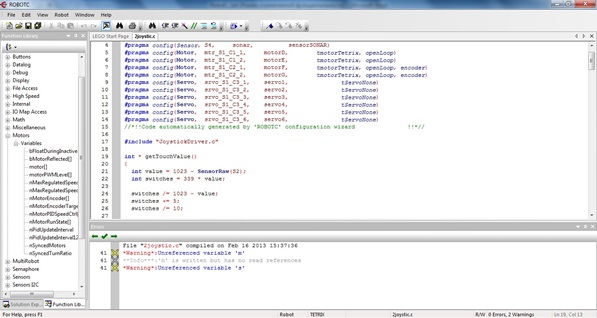
\includegraphics[width=0.93\linewidth]{chapters/chapter9/images/2}
		\caption{Вид текстового редактора RobotC.}
		\label{ris:image9x2}
	\end{center}
\end{figure}

Давайте напишем первую программу и заставим блок её исполнять. Вам необходимо создать текстовый файл с исходным кодом, скомпилировать его и подсунуть полученный бинарный файл микроконтроллеру в блоке.\\\\

{\hypertarget{lesson9x6}{\blackBlueText{VI. Практикум «Ленивая программа»}}}\\\\

Наша первая программа  будет самой ленивой программой, она не будет делать ничего, просто начнется и закончится. Нажмем на иконку  New  и создадим новый документ.

\begin{figure}[h!]
	\begin{center}
		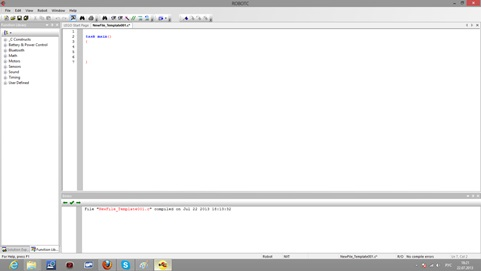
\includegraphics[width=1\linewidth]{chapters/chapter9/images/3}
		\caption{Новый документ в RobotC.}
		\label{ris:image9x3}
	\end{center}
\end{figure}

Основное отличие RobotC от C/C++ в том, что название главного оператора (функции с которой начинается компиляция~--- main) имеет тип “task”, то есть полная шапка функции будет иметь вид\\\\

{\programm
	{\slshape\bC{task main}}\rC{()}\\
	\rC{\{}\\\\
	\rC{\}}\\
}\\\\

Теперь программу надо скомпилировать и загрузить на микроконтроллер робота. Для этого сначала нажимаем F7 ( Robot\(\to\)Compile program). В окне вывода информации о компиляции  появляется надпись:

\begin{center}
	File "NewFile\_Template001.c" compiled on Jul 22 2013 17:07:10 
\end{center}

Это значит, что наша программа написана без ошибок и компилятор смог перевести ее на понятный процессору язык. Важно обратить внимание на то, что «без ошибок»~--- это не значит, что программа правильная и  будет делать то, что мы хотели. Это всего лишь значит, что написанный код возможно исполнить, к чему это приведет~--- пока неизвестно.

Теперь необходимо обновить прошивку робота, потому что разные версии IDE RobotC работают с различными не совместимыми с остальными версиями прошивками. При попытке отправить на робот код, скомпилированный под другую версию прошивки~--- возникнет ошибка.

Для перепрошивки (загрузки на робот прошивки) робота необходимо подсоединить блок с помощью USB кабеля с компьютером, зайти в пункт меню {\bfseries Robot\(\to\)Download Firmware} и выбрать пункт меню {\bfseries Standard File} и в появившемся окошке нажать на пункт {\bfseries F/W Download}.

\begin{figure}[h!]
	\begin{center}
		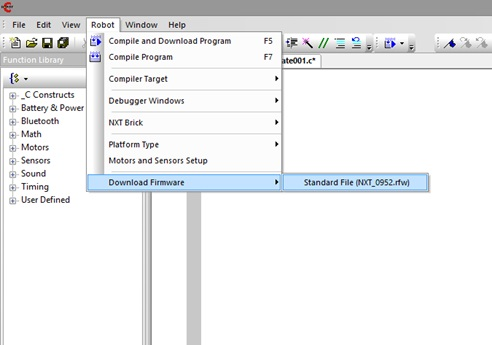
\includegraphics[width=1\linewidth]{chapters/chapter9/images/4}
		\caption{Прошивка робота.}
		\label{ris:image9x4}
	\end{center}
\end{figure}

После удачной перепрошивки робот включится. Во время перепрошивки ни в коем случае нельзя вынимать из блока батарейки, или же разрывать соединение блока с компьютером. Если же все же процесс перепрошивки был прерван, то его можно повторить, даже если робот не включается.

Теперь программу надо загрузить на включенного робота. Для этого выбираем {\bfseries Robot\(\to\)Compile and Download program}.Теперь на самом блоке можно выбрать программу и нажать Run. Ничего не произошло, но мы увидели как на экране мелькнула надпись End program. Наша первая программа ничего не сделала, но была успешно исполнена и завершилась. 

Прежде чем написать более сложную программу попробуем понять, зачем нам понадобилось писать столько строк, для программы, которая ничего не делает. Во-первых, оказывается что, компьютер всегда начинает чтение программы с определенного, главного блока, в независимости от того каким по порядку вы его написали. В  RobotC  эта функция, с которой начинается компиляция (главный оператор) носит название main и имеет тип task, указывающийся перед ней. Начало блока кода в RobotC обозначается левой фигурной скобкой \{, его конец~--- правой фигурной скобкой \}.Т.е. в переводе на русский мы написали примерно следующее:
\begin{itemize}
	\renewcommand{\textbullet}{\textendash}
	\item Начни читать программу отсюда
	\item Начало программы
	\item Конец программы
\end{itemize}

Итак, понадобилось три строчки, что бы робот ничего не сделал, но не сделал это грамотно. На следующем занятии робот научится ехать прямо. Подумаешь, это еще в Занятии 4 было реализовано. Но помимо этого робот научится проезжать заранее заданное расстояние. О, это уже интереснее.